%% abtex2-modelo-projeto-pesquisa.tex, v-1.9.7 laurocesar
%% Copyright 2012-2018 by abnTeX2 group at http://www.abntex.net.br/ 
%%
%% This work may be distributed and/or modified under the
%% conditions of the LaTeX Project Public License, either version 1.3
%% of this license or (at your option) any later version.
%% The latest version of this license is in
%%   http://www.latex-project.org/lppl.txt
%% and version 1.3 or later is part of all distributions of LaTeX
%% version 2005/12/01 or later.
%%
%% This work has the LPPL maintenance status `maintained'.
%% 
%% The Current Maintainer of this work is the abnTeX2 team, led
%% by Lauro César Araujo. Further information are available on 
%% http://www.abntex.net.br/
%%
%% This work consists of the files abntex2-modelo-projeto-pesquisa.tex
%% and abntex2-modelo-references.bib
%%

% ------------------------------------------------------------------------
% ------------------------------------------------------------------------
% abnTeX2: Modelo de Projeto de pesquisa em conformidade com 
% ABNT NBR 15287:2011 Informação e documentação - Projeto de pesquisa -
% Apresentação 
% ------------------------------------------------------------------------ 
% ------------------------------------------------------------------------
\documentclass[
	% -- opções da classe memoir --
	12pt,				% tamanho da fonte
	openright,			% capítulos começam em pág ímpar (insere página vazia caso preciso)
	twoside,			% para impressão em recto e verso. Oposto a oneside
	a4paper,			% tamanho do papel. 
	% -- opções da classe abntex2 --
	%chapter=TITLE,		% títulos de capítulos convertidos em letras maiúsculas
	%section=TITLE,		% títulos de seções convertidos em letras maiúsculas
	%subsection=TITLE,	% títulos de subseções convertidos em letras maiúsculas
	%subsubsection=TITLE,% títulos de subsubseções convertidos em letras maiúsculas
	% -- opções do pacote babel --
	english,			% idioma adicional para hifenização
	french,				% idioma adicional para hifenização
	spanish,			% idioma adicional para hifenização
	brazil,				% o último idioma é o principal do documento
	]{abntex2}

% ---
% PACOTES
% ---

% ---
% Pacotes fundamentais 
% ---
\usepackage{helvet}			% Usa a fonte Helvetica
\renewcommand{\familydefault}{\sfdefault} 
\usepackage[T1]{fontenc}		% Selecao de codigos de fonte.
\usepackage[utf8]{inputenc}		% Codificacao do documento (conversão automática dos acentos)
\usepackage{indentfirst}		% Indenta o primeiro parágrafo de cada seção.
\usepackage{color}				% Controle das cores
\usepackage{graphicx}			% Inclusão de gráficos
% caminho para a pasta de imagens
\graphicspath{ {imagens/} }
\usepackage{fancyvrb}
%\usepackage{microtype} 			% para melhorias de justificação
\usepackage[nonumberlist=true, 
					toc,
					style=index,
					translate=babel,
					automake]{glossaries}
%\makeglossaries
% ---

% ---
% Pacotes adicionais, usados apenas no âmbito do Modelo Canônico do abnteX2
% ---
% ---
% Pacotes de citações
% ---
\usepackage[brazilian,hyperpageref]{backref}	 % Paginas com as citações na bibl
\usepackage[alf, abnt-emphasize=bf, bibjustif]{abntex2cite}	% Citações padrão ABNT
\usepackage[table,xcdraw]{xcolor} % Permite a colorizaão da tabela do cronograma
\usepackage{lscape} % Permite a impressão de páginas em modo paisagem 
\usepackage{hyperref}
\usepackage{diagbox}
\usepackage{verbatim}
\usepackage{pdfpages} % Permite a inserção de arquivos pdf no documento final
\usepackage{url}
\usepackage{glossaries}
\def\UrlBreaks{\do\/\do-}


% --- 
% CONFIGURAÇÕES DE PACOTES
% --- 

% ---
% Configurações do pacote backref
% Usado sem a opção hyperpageref de backref
\renewcommand{\backrefpagesname}{Citado na(s) página(s):~}
% Texto padrão antes do número das páginas
\renewcommand{\backref}{}
% Define os textos da citação
\renewcommand*{\backrefalt}[4]{
	\ifcase #1 %
		Nenhuma citação no texto.%
	\or
		Citado na página #2.%
	\else
		Citado #1 vezes nas páginas #2.%
	\fi}%
% ---

% ---
% Informações de dados para CAPA e FOLHA DE ROSTO
% ---

\titulo{Edite o arquivo dados.tex para colocar os dados da capa, folha de rosto e aprovação}
\autor{Nome do autor}
\local{Cidade do Autor - PI}
\data{mês e ano}
\instituicao{%
  UNIVERSIDADE FEDERAL DO PIAUÍ -- UFPI
  \par
  CENTRO DE EDUCAÇÃO ABERTA E A DISTÂNCIA – CEAD/UFPI
  \par
  CURSO DE BACHARELADO EM SISTEMAS DE INFORMAÇÃO}
\tipotrabalho{Trabalho de Conclusão de Curso}
% O preambulo deve conter o tipo do trabalho, o objetivo, 
% o nome da instituição e a área de concentração 
\preambulo{Monografia submetida ao Curso de Bacharelado de Sistemas de Informação como requisito parcial para obtenção de grau de Bacharel em Sistemas de Informação.}
\orientador{Nome do Orientador}
% Comente a linha abaixo com '%' se não houver coorientador
\coorientador{Nome do Coorientador}
% ---
% Para multiplos coorientadores use a seguinte alternativa:
% \coorientador{Nome do Coorientador 1\par Coorientador: Nome do Coorientador 2}
% ---

\loadglsentries{postextuais/glossarios} %Carrega as entradas do glossário, se existirem
\makeglossaries

% ---
% Configurações de aparência do PDF final
% ---


% ----e um
% INICIO DAS CUSTOMIZACOES PARA A UNIVERSIDADE FEDERAL DO PIAUÍ
% ---

\newcommand{\capaufpi}{%
	\begin{capa}%
		\center
		\textbf{\normalsize\imprimirinstituicao}
		
		\vfill
		\begin{vplace}[0.2]
			\textbf
			{\large{MONOGRAFIA}}
			%	    \vspace*{1.0cm}
			\vfill
			\textbf{\center\LARGE\imprimirtitulo}
			\vfill		     
			%	    \vspace{2cm}
			\textbf{\large\imprimirautor}
		\end{vplace}
		
		\vfill
		
		\textbf{\normalsize\imprimirlocal}
		
		\textbf{\normalsize\imprimirdata}
		
		\vspace*{1cm}
		
	\end{capa}
}


% folha de rosto 

\makeatletter

\newcommand{\frostoUFPI}{
\begin{center}
	%\large\imprimirinstituicao
    
%    \vspace*{1cm}
    
{\large\imprimirautor}

\vspace*{\fill}\vspace*{\fill}

\begin{center}
\bfseries\Large\imprimirtitulo
\end{center}

\vspace*{\fill}

\abntex@ifnotempty{\imprimirpreambulo}{%
  \hspace{.45\textwidth}
  \begin{minipage}{.5\textwidth}
  \SingleSpacing
  \imprimirpreambulo
  \par
  \vspace{1cm}
  \imprimirorientadorRotulo~\imprimirorientador\par
  \imprimircoorientadorRotulo~\imprimircoorientador
  \end{minipage}%
  \vspace*{\fill}
}%



	\vspace*{\fill}


	{\large\imprimirlocal}

	\par

	{\large\imprimirdata}
	\vspace*{1cm}
\end{center}
}

\makeatother

% ---
% FIM DAS CUSTOMIZACOES PARA A UNIVERSIDADE FEDERAL DO PIAUÍ
% ---

% alterando o aspecto da cor azul
\definecolor{blue}{RGB}{41,5,195}

% informações do PDF
\makeatletter
\hypersetup{
     	%pagebackref=true,
		pdftitle={\@title}, 
		pdfauthor={\@author},
    	pdfsubject={\imprimirpreambulo},
	    pdfcreator={LaTeX with abnTeX2},
		pdfkeywords={abnt}{latex}{abntex}{abntex2}{projeto de pesquisa}, 
		colorlinks=true,       		% false: boxed links; true: colored links
    	linkcolor=blue,          	% color of internal links
    	citecolor=blue,        		% color of links to bibliography
    	filecolor=magenta,      		% color of file links
		urlcolor=blue,
		bookmarksdepth=4
}
\makeatother
% --- 

% --- 
% Espaçamentos entre linhas e parágrafos 
% --- 

% O tamanho do parágrafo é dado por:
\setlength{\parindent}{1.3cm}

% Controle do espaçamento entre um parágrafo e outro:
\setlength{\parskip}{0.2cm}  % tente também \onelineskip

% ---
% compila o indice
% ---
\makeindex
% ---
% ----
% Início do documento
% ----
\begin{document}

% Seleciona o idioma do documento (conforme pacotes do babel)
%\selectlanguage{english}
\selectlanguage{brazil}

% Retira espaço extra obsoleto entre as frases.
\frenchspacing 

% ----------------------------------------------------------
% ELEMENTOS PRÉ-TEXTUAIS
% ----------------------------------------------------------
% \pretextual

% ---
% Capa
% ---
%\imprimircapa
\capaufpi
% ---

% ---
% Folha de rosto
% ---
%\imprimirfolhaderosto
\frostoUFPI
% ---

% ---
% Após a aprovação pela banca o documento deve ser catalografado pela Biblioteca da UFPI. Após a solicitação
% do serviço ela deve ser inserida imediatamente após a ata de aprovação. Para preparar para a versão final 
% você deverá incluir o arquivo na página pretextuais e mudar seu nome para ficha_catalografica.pdf e 
% descomentar a linha a seguir
% ---
% 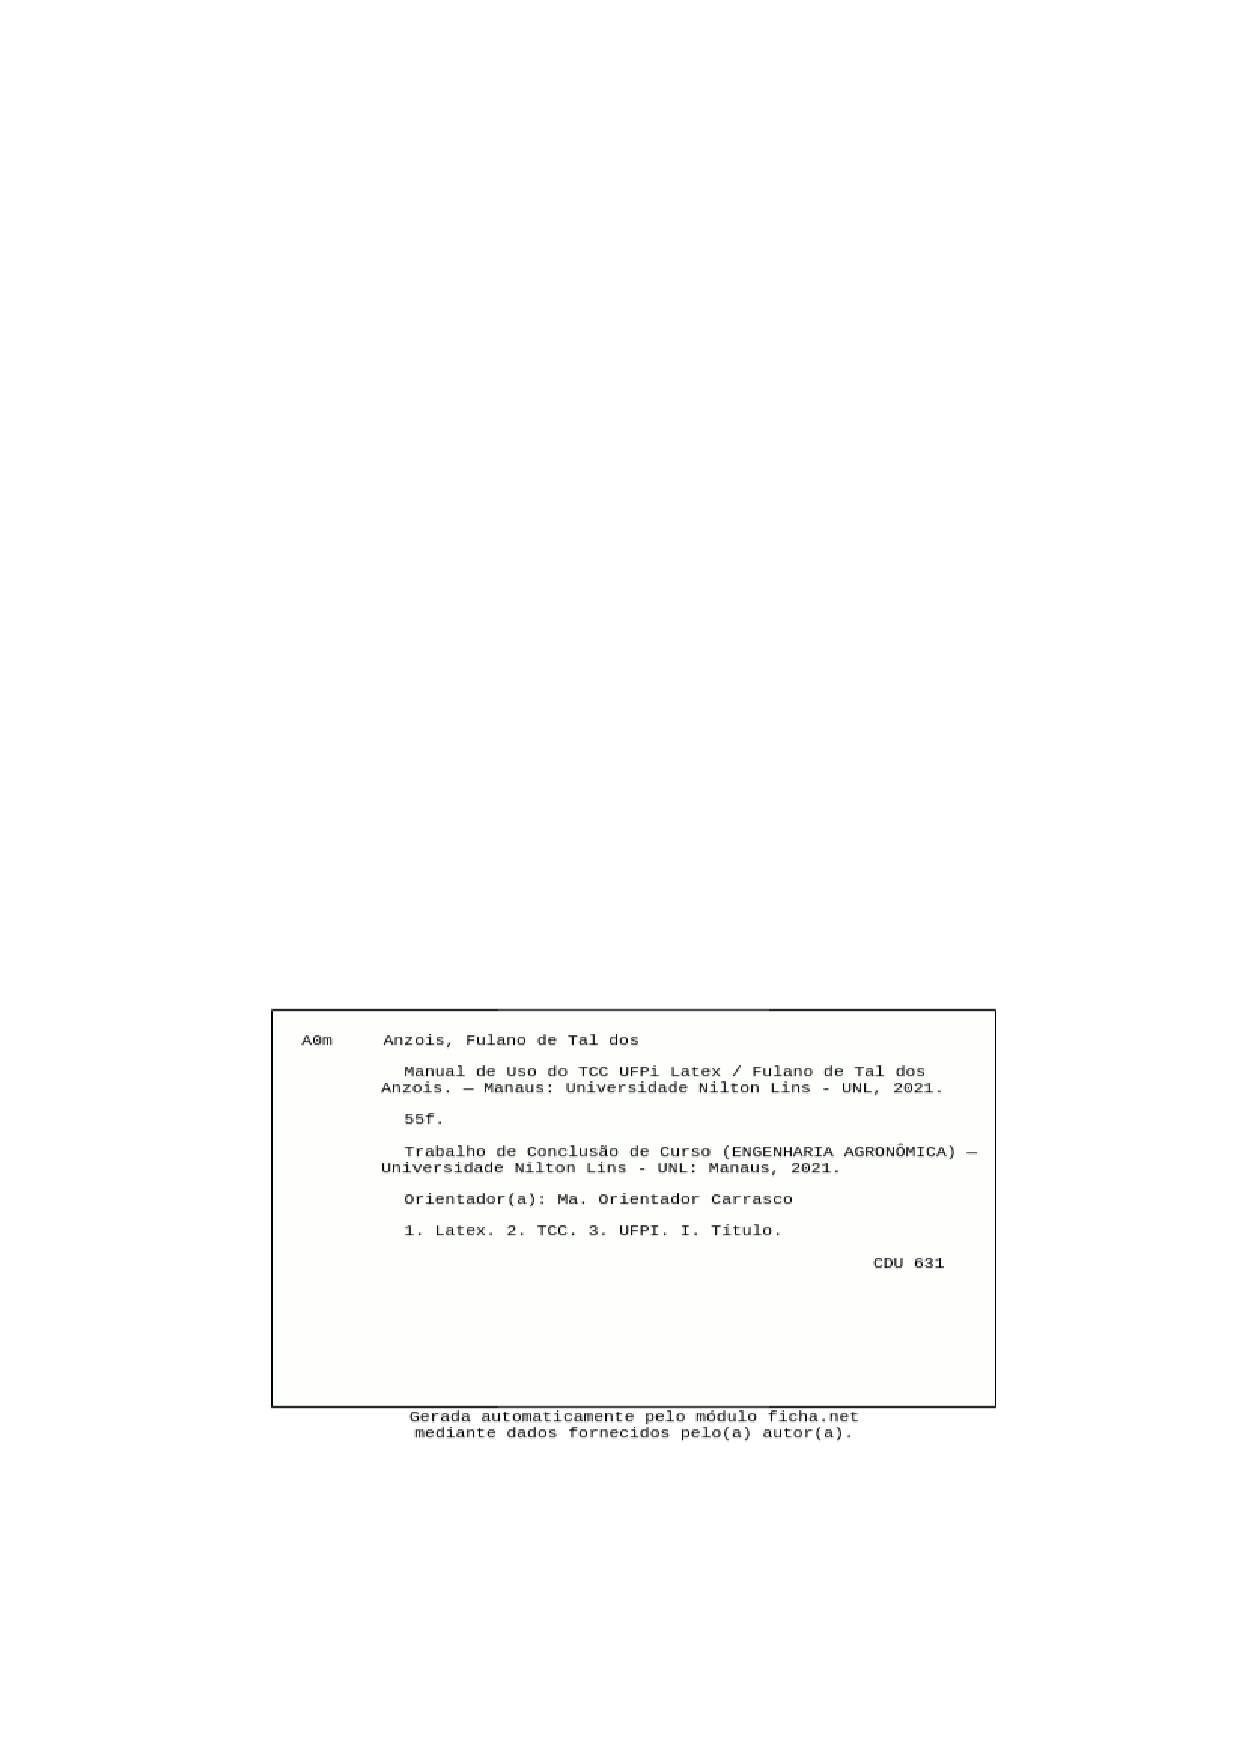
\includepdf[pages=-]{pretextuais/ficha_catalografica.pdf}

% ---
% A folha de aprovação deve ser inclusa a versão entregue antes da defesa, após a defesa ela
% será substituida pela ata de aprovação, assinada pela banca.
% ---
% ================================================================================
% Modelo da folha de aprovação, padrão UFPI, conforme modelo 
% disponível em https://drive.google.com/file/d/0B0BKqBVXhtedLWQzYVBhbUNRT1U/edit
% ================================================================================

\begin{folhadeaprovacao}
\begin{center}
	{\ABNTEXchapterfont\large\imprimirautor}
	\vspace*{\fill}\vspace*{\fill}
	\begin{center}
		\ABNTEXchapterfont\bfseries\Large\imprimirtitulo
	\end{center}
	\vspace*{\fill}
	\hspace{.45\textwidth}
	\begin{minipage}{.5\textwidth}
		\imprimirpreambulo
	\end{minipage}%
	\vspace*{\fill}
\end{center}

Trabalho \rule{4cm}{1pt}. \imprimirlocal, \rule{1cm}{1pt} de \rule{3cm}{1pt} de 2020:

% ===
% edite os nomes e cargos dos professores da banca
% ===
\assinatura{\textbf{\imprimirorientador} \\ Orientador}
\assinatura{\textbf{Nome do coorientador} \\ Coorientador}
\assinatura{\textbf{Professor} \\ Convidado 1}
\assinatura{\textbf{Professor} \\ Convidado 2}
\assinatura{\textbf{Professor} \\ Convidado 3}
\begin{center}
	\vspace*{0.5cm}
	{\large\imprimirlocal}
	\par
	{\large\imprimirdata}
	\vspace*{1cm}
\end{center}
\end{folhadeaprovacao} % Coloque um % no começo dessa linha para emitir a folha de aprovação

% ---
% A ata de aprovação será entregue pela banca após a defesa. Ela deve constar na versão final do documento
% impresso. Você pode inserir ela no documento copiando o arquivo para a pasta pretextuais e mudando seue nome
% para ata.pdf e descompentando a linha abaixo
% ---
% \includepdf[pages=-]{pretextuais/ata.pdf}







% ---
% NOTA DA ABNT NBR 15287:2011, p. 4:
%  ``Se exigido pela entidade, apresentar os dados curriculares do autor em
%     folha ou página distinta após a folha de rosto.''
% ---

% ---
% inserir lista de ilustrações
% ---
\pdfbookmark[0]{\listfigurename}{lof}
\listoffigures*
\cleardoublepage
% ---

% ---
% inserir lista de tabelas
% ---
%\pdfbookmark[0]{\listtablename}{lot}
\listoftables*
\cleardoublepage
% ---

% ---
% inserir lista de abreviaturas e siglas
% Edite o arquivo siglas.tex na pasta pretextuais
% ---
\begin{siglas}
  \item[UFPI] Universidadde Federal do Piauí
  \item[CEAD] Centro de Educação Aberta e a Distância
\end{siglas}
% ---

% ---
% inserir lista de símbolos
% ---
%\begin{simbolos}
%  \item[$ \Gamma $] Letra grega Gama
%  \item[$ \Lambda $] Lambda
%  \item[$ \zeta $] Letra grega minúscula zeta
%  \item[$ \in $] Pertence
%\end{simbolos}
% ---

% ---
% inserir o sumario
% ---
\pdfbookmark[0]{\contentsname}{toc}
\tableofcontents*
\cleardoublepage
% ---

% ----------------------------------------------------------
% ELEMENTOS TEXTUAIS
% ----------------------------------------------------------
\textual
% ----------------------------------------------------------
% Os includes a seguir incluirão os arquivos contidos na pasta 
% textuais e poderão ou não ser omitidos.  
% ----------------------------------------------------------
\begin{resumo}
	%Resumo
	\vspace{\onelineskip}
	\noindent
	Para editar o resumo edite o arquivo resumo.tex na pasta textuais. 
	\par\textbf{Palavras-chave}: resumo, latex
\end{resumo}



\begin{resumo}[Abstract]
\begin{otherlanguage*}{english}  
	\vspace{\onelineskip}
	\noindent
		%---------------------
		% Edite a partir daqui 
		%---------------------
		To edit the abstract, edit the file abstract.tex in the textuais folder. 
		\par\textbf{Keywords}: latex, UFPI.
\end{otherlanguage*}
\end{resumo}
\chapter{Introdução}
%---------------------
% Edite a partir daqui 
%---------------------
Para editar a introdução, edite o arquivo introdução.tex na pasta textuais. Para chamar uma entrada do \gls{gls} use \verb+\gls{rótulo}+, chamando a entrada apropriada no arquivo postextuais/glossarios.tex.
\chapter{Justificativa}
%---------------------
% Edite a partir daqui 
%---------------------
Para editar a justificativa, edite o arquivo justificativa.tex na pasta textuais. 
\chapter{Problematização}
%---------------------
% Edite a partir daqui 
%---------------------
Para editar a problematização, edite o arquivo problematização.tex na pasta textuais. 
\chapter{Hipotese}
%---------------------
% Edite a partir daqui 
%---------------------
Para editar a hipotese, edite o arquivo hipotese.tex na pasta textuais. 
\chapter{Objetivos}
%---------------------
% Edite a partir daqui 
%---------------------

Para editar os objetivos, edite o arquivo objetivos.tex. 


\begin{itemize}
	\item Este é um modelo de lista não-numerada.
\end{itemize}



\chapter{Revisão Bibliográfica}
%---------------------
% Edite a partir daqui 
%---------------------
Para editar a revisão bibliográfica edite o arquivo revisão.tex na pasta textuais. 
\par
Para criar a lista de referência recomendo criar um arquivo bibtex )referencias.bib) no Mendeley, Jabref, bibtex.online, ou outro gerenciador de referências, ou ainda criar as referências a partir dos geradores de sites como Google Scholar, Periodicos Capes, etc. 
\par
Para citar no estilo (AUTOR, 2000) use \verb+\cite{id da referência}+
\par
Por exemplo: \cite{Abuidris2019}
\par
Para citar no estilo Autor (2000) use \verb+\citeonlin{id da referência}+
\par
Por exemplo: \citeonline{Ufpi2020}
\par
As ids de referências são as existentes no começo de cada entrada do arquivo bibtex. As citações criam as referências automaticamente no fim do texto, somente aquelas existentes no arquivo referencia.bib e efetivamente usadas aparecerão na seção correspondente.

Para criar apêndices e anexos, edite a parte correspondente no arquivo TCC1.tex, removendo os comentários \verb+%+ nos comandos \verb+\partapendices+ e \verb+\partanexos+ da seção postextuais, e incluindo os arquivos pertinentes na pasta postextuais.

\chapter{Metodologia}
%---------------------
% Edite a partir daqui 
%---------------------
Para alterar a metodologia, edite o arquivo metodologia.tex na pasta textuais. 
 % O conteúdo deste arquivo pode ser incluído na proposta de trabalho
\chapter{Cronograma}
%---------------------
% Edite a partir daqui 
%---------------------
Para editar o cronograma você deve editar o arquivo cronograma.tex na pasta textuais. No entanto recomendo usar um editor de tabelas para latex. 
\begin{table}[h]
	\centering
	\small
	\begin{tabular}{|l|l|l|l|l|l|l|l|} 
		\hline
		& Ago 2020 & Set 2020 & Out 2020 & Nov 2020 & Dez 2020 & Jan 2021 & Fev 2020  \\ 
		\hline
		\begin{tabular}[c]{@{}l@{}}Desenhar e \\prototipar o \\sistema\end{tabular} & \cellcolor{blue!25}          &          &          &          &          &          &           \\ 
		\hline
		\begin{tabular}[c]{@{}l@{}}Implementar o \\sistema\end{tabular}             &          & \cellcolor{blue!25}         &          &          &          &          &           \\ 
		\hline
		\begin{tabular}[c]{@{}l@{}}Realizar eleições \\simuladas\end{tabular}     &          &          &  \cellcolor{blue!25}        & \cellcolor{blue!25}         &          &          &           \\ 
		\hline
		\begin{tabular}[c]{@{}l@{}}Coletar dados\end{tabular}                    &          &          & \cellcolor{blue!25}         & \cellcolor{blue!25}         &          &          &           \\ 
		\hline
		\begin{tabular}[c]{@{}l@{}}Analisar dados\end{tabular}                   &          &          &          &          & \cellcolor{blue!25}         &          &           \\ 
		\hline
		\begin{tabular}[c]{@{}l@{}}Escrever \\a monografia\end{tabular}             &          &          &          &          &  \cellcolor{blue!25}        &  \cellcolor{blue!25}        &           \\ 
		\hline
		\begin{tabular}[c]{@{}l@{}}Defender \\a monografia\end{tabular}             &          &          &          &          &          &          & \cellcolor{blue!25}           \\
		\hline
	\end{tabular}
\end{table}
 % Este arquivo é exclusivo do TCC 2, para retira-lo coloque um % no começo da linha
\chapter{Proposta de Trabalho}
O conteúdo deste capitulo poderá ser mesclado ou não com o capítulo metodologia. Para alterar o conteúdo deste capitulo edite o arquivo \verb|textuais/proposta.tex| % Este arquivo é exclusivo do TCC 2, para retira-lo coloque um % no começo da linha
\chapter{Resultados}

Para editar o conteúdo deste capitulo altere o arquivo \verb|textuais/resultados.tex|  % Este arquivo é exclusivo do TCC 2, para retira-lo coloque um % no começo da linha
\chapter{Discussão}

Este arquivo pode ou não estar agregado aos resultados, consulte seu orientador quanto a isso. Para editar o texto desta sessão altere o arquivo \verb|textuais/discussao.tex|. % Este arquivo é exclusivo do TCC 2, para retira-lo coloque um % no começo da linha
\chapter{Conclusão}
Para editar o conteúdo deste capítulo altere o conteúdo do arquivo \verb|textuais/conclusao.tex|. % Este arquivo é exclusivo do TCC 2, para retira-lo coloque um % no começo da linha


% ----------------------------------------------------------
% Capitulo com exemplos de comandos inseridos de arquivo externo 
% ----------------------------------------------------------

%\include{abntex2-modelo-inclCitaude-comandos}

% ---
% Finaliza a parte no bookmark do PDF
% para que se inicie o bookmark na raiz
% e adiciona espaço de parte no Sumário
% ---
\phantompart

% ---
% Conclusão
% ---

% ----------------------------------------------------------
% ELEMENTOS PÓS-TEXTUAIS
% ----------------------------------------------------------
\postextual

% ----------------------------------------------------------
% Referências bibliográficas
% ----------------------------------------------------------
\bibliography{postextuais/referencias}

% ----------------------------------------------------------
% Glossário
% ----------------------------------------------------------
%
% Consulte o manual da classe abntex2 para orientações sobre o glossário.
%

%\printglossaries

\glossary{postextuais/glossarios}
\printglossaries

% ----------------------------------------------------------
% Apêndices
% ----------------------------------------------------------

% ---
% Inicia os apêndices
% ---
\begin{apendicesenv}
	
\chapter{Observações sobre apêndices}

Apêndices são conteúdos originais produzidos por você, como texto, código fonte, uma imagem, etc. e que não são citados diretamente no texto principal e servem para complementar a argumentação. O conteúdo dos apêndices é basicamente igual a um capítulo do texto principal, inicia com \verb|\chapter{Nome do apêndice}|. 

Cada apêndice deve ser incluído entre o \verb|\begin{apendicesenv}| e \verb|\end{apendicesenv}| com o comando \verb|\include{postextuais/nomedoarquivo|, sem a extensão \verb|.tex|. Os arquivos devem estar na pasta postextuais.

% Imprime uma página indicando o início dos apêndices
% ↓ Remova o '%' para imprimir o inicio da parte dos apêndices
%\partapendices

% O que for incluido por aqui até o end serão os aprendices

\end{apendicesenv}
% ---


% ----------------------------------------------------------
% Anexos
% ----------------------------------------------------------

% ---
% Inicia os anexos
% ---
\begin{anexosenv}

\chapter{Observações sobre anexos}

Anexos são conteúdos \textbf{não} produzidos por você, como texto, código fonte, uma imagem, etc. e que não são citados diretamente no texto principal e servem para complementar a argumentação. O conteúdo dos anexos é basicamente igual a um capítulo do texto principal, inicia com \verb|\chapter{Nome do apêndice}|. 

Cada anexo deve ser incluído entre o \verb|\begin{apendicesenv}| e \verb|\end{apendicesenv}| com o comando \verb|\include{postextuais/nomedoarquivo|, sem a extensão \verb|.tex|. Os arquivos devem estar na pasta postextuais.

% Imprime uma página indicando o início dos anexos
% ↓ Remova o '%' para imprimir o inicio da parte dos anexos
  %\partanexos
 
%O que for incluido por aqui até o end será considerado anexo

\end{anexosenv}

%---------------------------------------------------------------------
% INDICE REMISSIVO
%---------------------------------------------------------------------

\phantompart

\printindex


\end{document}
